\documentclass[../main/main.tex]{subfiles}

\begin{document}

\onlyinsubfile{%

}

% ==================================================================
% Section : Robustness
% ==================================================================
\section{Robustness}
\label{sec:robustness}

\begin{frame}{Robustness - Outline}
  \tableofcontents[currentsection, hideothersubsections]
\end{frame}
% ==================================================================

% ==================================================================
\subsection{Classical margins}
\begin{frame}{Are the classical control margins are really adapted?}
  \begin{columns}
    \begin{column}{0.7\textwidth}
      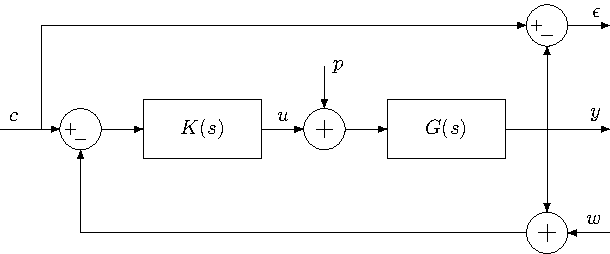
\includegraphics[width=1.0\textwidth, height=0.9\textheight, keepaspectratio]{h-infinity-variables}\\\vspace{1em}
      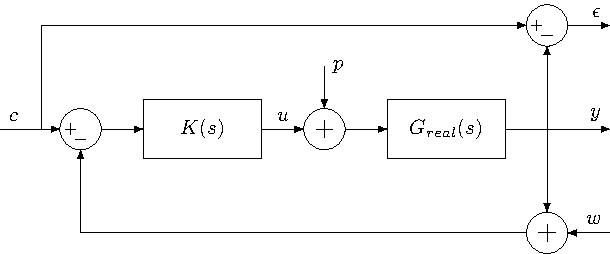
\includegraphics[width=1.0\textwidth, height=0.9\textheight, keepaspectratio]{h-inf-g-reel}
    \end{column}
    \begin{column}{0.3\textwidth}
      \[ G \neq G_{real} \]
      How can we be sure about the robustness in performances and the \textbf{robustenes in stability}?
    \end{column}
  \end{columns}
\end{frame}

\begin{frame}{Classical Margins: Gain and Phase}
  \begin{columns}
    \begin{column}{0.6\textwidth}
      \stitle{Nyquist plot}\\\vspace{1em}
      \begin{overprint}
        \onslide<1>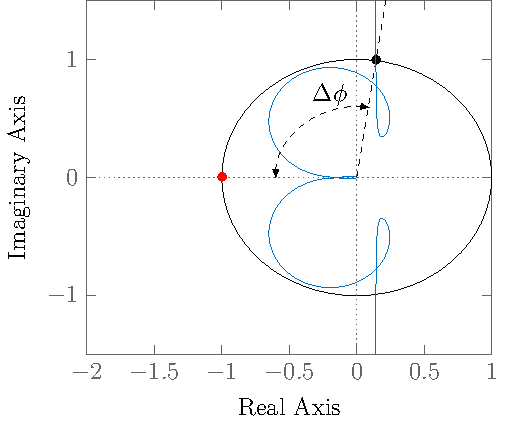
\includegraphics[width=1.0\textwidth, height=0.9\textheight, keepaspectratio]{phase-margin}
        \onslide<2>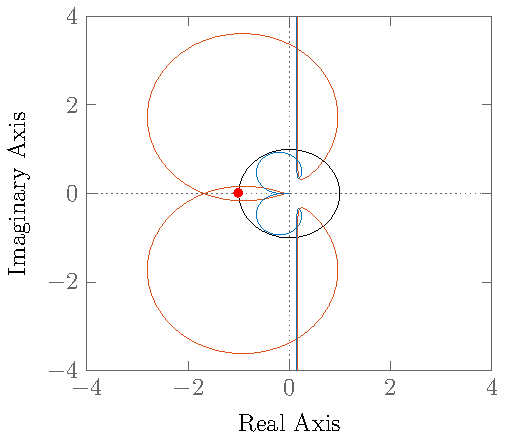
\includegraphics[width=1.0\textwidth, height=0.9\textheight, keepaspectratio]{phase-margin-bis}
      \end{overprint}
    \end{column}
    \begin{column}{0.4\textwidth}
      \begin{align*}
        L(s) & = K(s) G(s)\\
             & = \text{Open Loop TF}
      \end{align*}
      \onslide<1->{\color{mycolor1}
        \[ L(s) = \frac{0.07(s+7.5)(s+2)}{s(s^2 + 0.4s+4)} \]
      }

      \onslide<2>{\color{mycolor2}
        \[ L(s) = \frac{0.07(s+7.5)(s+2)}{s(s^2 + \boldsymbol{0.152}s+4)} \]
      }
    \end{column}
  \end{columns}
\end{frame}
% ==================================================================

% ==================================================================
\subsection{Module Margin}

\begin{frame}{Module Margin}
  \begin{columns}
    \begin{column}{0.5\textwidth}
      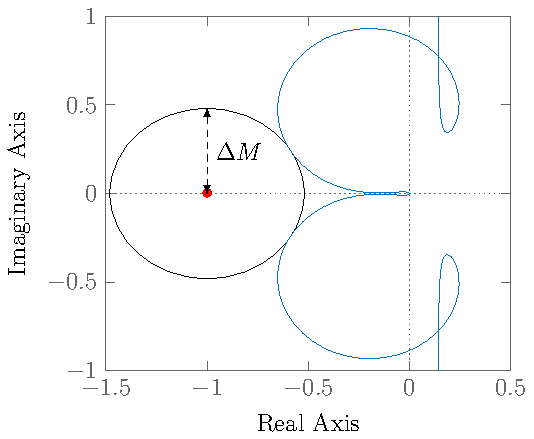
\includegraphics[width=1.0\textwidth, height=0.9\textheight, keepaspectratio]{module-margin}
    \end{column}
    \begin{column}{0.5\textwidth}
      % TODO: should talk about h infinity norm before that
      \begin{align*}
        \Delta M & = min_{\omega}\abs{1+L(j\omega)}\\
                 & = \frac{1}{sup_\omega\frac{1}{\norm{1+L(j\omega)}}}\\
                 & = \frac{1}{\hnorm{S}}
      \end{align*}
    \end{column}
  \end{columns}
  \begin{tcolorbox}[size=small, top=4pt, colback=red!5!white,colframe=red!75!black,title=If we want to have a good module margin]
    $\forall \omega, \Vert T_{c\rightarrow\epsilon}(j\omega)\Vert < \Delta M_{\text{min}}$ Usually we can take $M_{\text{min}} = 0.5$
  \end{tcolorbox}
\end{frame}

\begin{frame}{Weighting Functions}
  \centering
  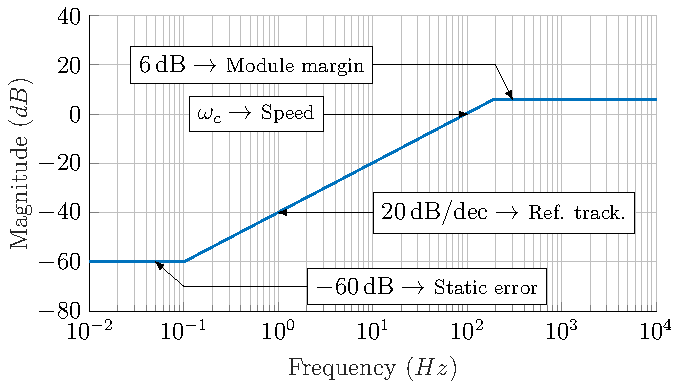
\includegraphics[width=1.0\textwidth, height=0.9\textheight, keepaspectratio]{contr_W1}
\end{frame}
% % ==================================================================


% Peut être mettre ça dans la partie sur la robustesse
\begin{frame}[t]{Optimal control against disturbances}
  LQG: disturbance attenuation problem: magnitude of the output is minimized
  subject to appropriate assumption on the disturbances.
  \[ J_2 = \lim_{t_f \rightarrow \infty} E \left[ \frac{1}{t_f} \int_0^{t_f}z^\intercal(t)z(t)dt\right] \]
  $J_2$ is equal to the norm \(H_2\) of the closed loop transfert function:
  it's $H_2$-optimal control.
  Definition norm \(H_2\): \[\twonorm{G} = ( \frac{1}{2\pi} \int_{-\infty}^{\infty}\vert G(j\omega)\vert^2 d\omega )^{1/2}\]
  % It's scalar that the average of the square of the gain taken over all frequencies
\end{frame}

\begin{frame}[t]{Robust control of uncertain plants}
  \begin{tcolorbox}[size=small, top=4pt,
    colback=blue!5!white,colframe=blue!75!black,title=Classical robustness against model uncertainties]
    Handled by phase and gain margin to ensure closed-loop stability in spite of modeling errors
    Problems:
    \begin{itemize}
    \item Not readily generaliwed to multivariable plants
    \item They do not handle the prolem of simultaneously achieving good
      performance against disturbances as well as robustness against model uncertainties
    \end{itemize}
  \end{tcolorbox} 
  $H_\infty$ norm of a stable tranfert function $G(s)$ is the largest gain the
  $G$ over all frequencies: \(\hnorm{G(s)} = \max_\omega{\vert G(j\omega) \vert}\)
\end{frame}





\end{document}

